\documentclass[11pt]{article}
\usepackage[margin=1in]{geometry}
\usepackage{enumitem}
\usepackage{hyperref}
\usepackage{graphicx}
\usepackage{array}
\usepackage{multicol}
\usepackage{longtable}
\usepackage{titlesec}
\usepackage{amsmath}
\usepackage{float}
\begin{document}

%==================================================
\begin{center}
    \large \textbf{Sri Sivasubramaniya Nadar College of Engineering, Chennai} \\
    (An Autonomous Institution Affiliated to Anna University) \\
    \vspace{0.3cm}
\end{center}
\begin{table}[h]
\renewcommand{\arraystretch}{1.4}
\resizebox{\textwidth}{!}{%
\begin{tabular}{|l|l|l|l|}
\hline
Degree \& Branch & B.E. Computer Science \& Engineering & Semester & VI \\ \hline
Subject Code \& Name & \multicolumn{3}{l|}{UCS2612 – Machine Learning Algorithms Laboratory} \\ \hline
Academic Year & 2025–2026 (Even) & Batch & 2023–2027 \\ \hline
Name & Kushaal Shyam Potta & Register No. & 3122235001071 \\ \hline
Due Date & \multicolumn{3}{l|}{24.01.2026} \\ \hline
\end{tabular}}
\end{table}


\begin{center}
\textbf{Experiment 4: Binary Classification using Linear and Kernel-Based Models}
\end{center}

%==================================================
\section*{Objective}
The primary goal of this study is to categorize emails into "spam" or "ham" (non-spam) categories by utilizing Logistic Regression and Support Vector Machine (SVM) algorithms. Additionally, the project aims to evaluate how systematic hyperparameter optimization impacts the classification accuracy and overall performance of these models.

%==================================================
\section*{Dataset}
The analysis utilizes the \textbf{Spambase} dataset, which consists of numerical attributes derived from the text of emails, alongside binary labels distinguishing between spam and non-spam messages.

\textbf{Dataset Link:}
\begin{itemize}
    \item Kaggle: \href{https://www.kaggle.com/datasets/somesh24/spambase}{https://www.kaggle.com/datasets/somesh24/spambase}
\end{itemize}

\section*{3. Preprocessing Steps}

To ensure the dataset was suitable for robust model training and validation, the following preprocessing methods were used.

\subsection*{3.1 Missing Value Check}
The dataset was screened for null or missing entries. The inspection confirmed that the data was complete due to which no processing techniques were necessary.

\subsection*{3.2 Feature Standardization}
All numerical input variables were normalized using StandardScaler to establish a mean of 0 and a standard deviation of 1. This step is critical for distance-sensitive algorithms like Support Vector Machines and Logistic Regression, as it prevents features with larger magnitudes from disproportionately influencing the model.

\subsection*{3.3 Train--Test Split}
The data was divided into training and testing subsets utilizing an 80:20 ratio. The training partition was employed to estimate model parameters, while the testing partition was set aside to assess the model's ability to generalize to new, unseen data.

\section*{4. Implementation Details}
All classification models were developed using the scikit-learn framework, incorporating the following configurations and optimization strategies.

\subsection*{4.1 Logistic Regression}
Logistic Regression classifiers were trained utilizing various solvers, specifically liblinear and saga. The study assessed the impact of both Lasso ($L1$) and Ridge ($L2$) regularization methods. To optimize the bias-variance tradeoff, the inverse regularization strength parameter, C, was tuned across a designated range of values.

\subsection*{4.2 Support Vector Machine (SVM)}
The SVM classifiers were tested using a diverse set of kernel functions: Linear, Polynomial, Radial Basis Function (RBF), and Sigmoid. Model selection involved hyperparameter tuning for the regularization term C (spanning 0.1 to 100), the kernel coefficient gamma (using both scale and auto modes), and the degree parameter for polynomial kernels.

\subsection*{4.3 Validation Technique}
To ensure the experimental results were consistent and robust, a 5-Fold Cross-Validation technique was applied during the hyperparameter tuning phase.


\section*{5. Visualizations}

\begin{figure}[H]
\centering
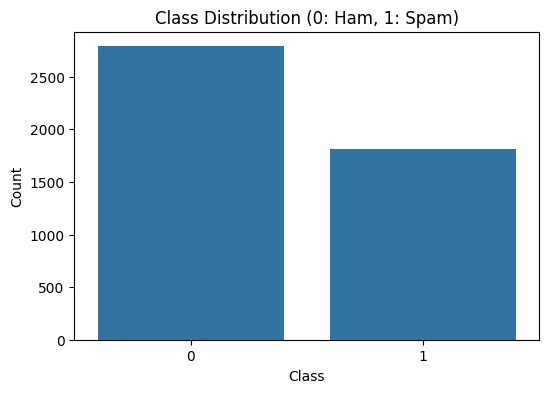
\includegraphics[width=0.65\textwidth]{spam_class_dist.png}
\caption{Class Distribution}
\end{figure}

\begin{figure}[H]
    \centering
    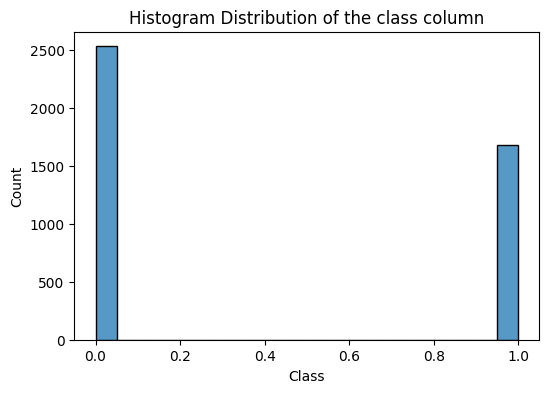
\includegraphics[width=0.5\linewidth]{spam_hist_dist.png}
    \caption{Histogram Distribution}
    \label{fig:placeholder}
\end{figure}

\begin{figure}[H]
\centering
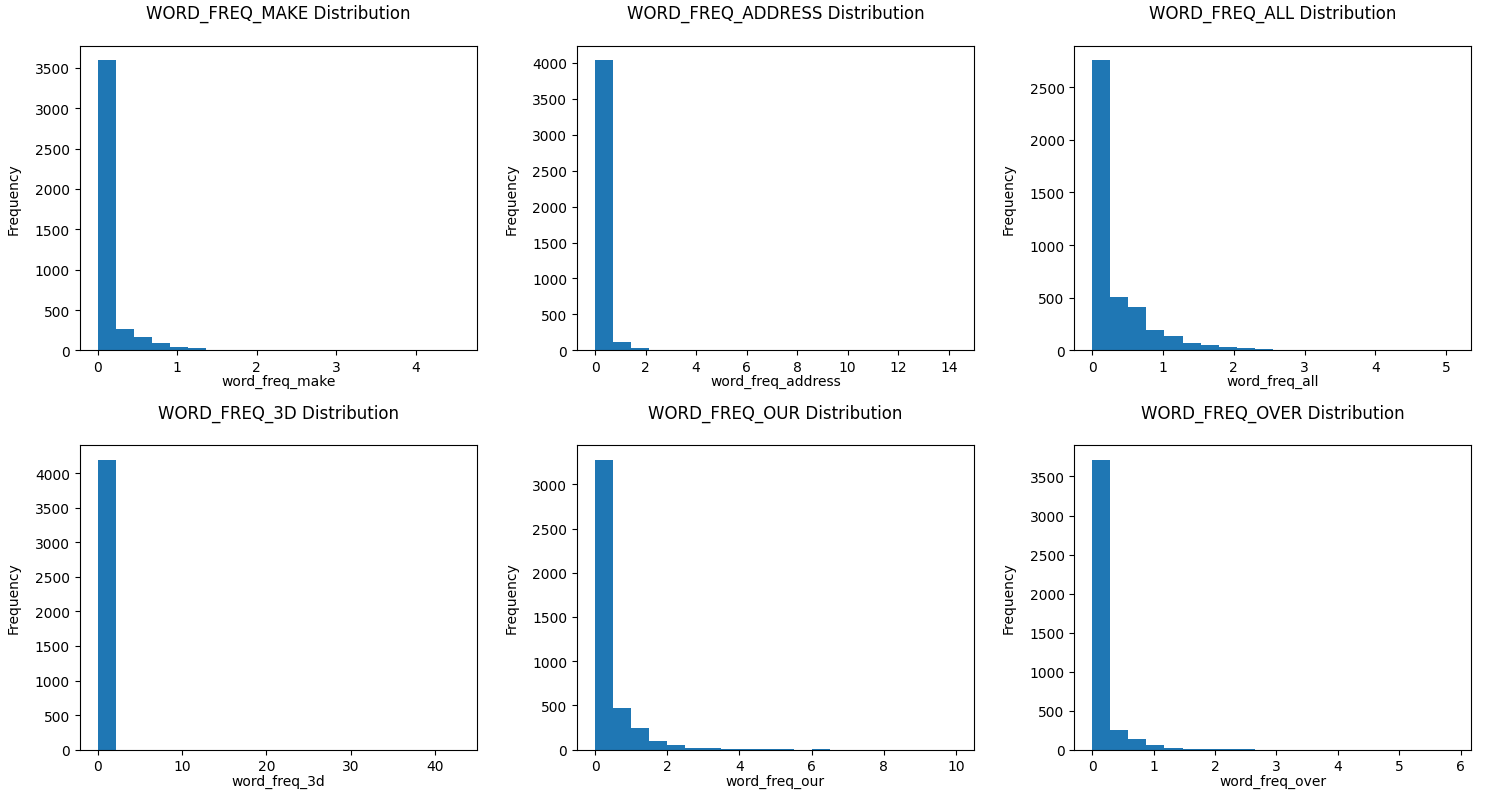
\includegraphics[width=0.85\textwidth]{spam_hist.png}
\caption{Histogram plot}
\end{figure}

\begin{figure}[H]
\centering
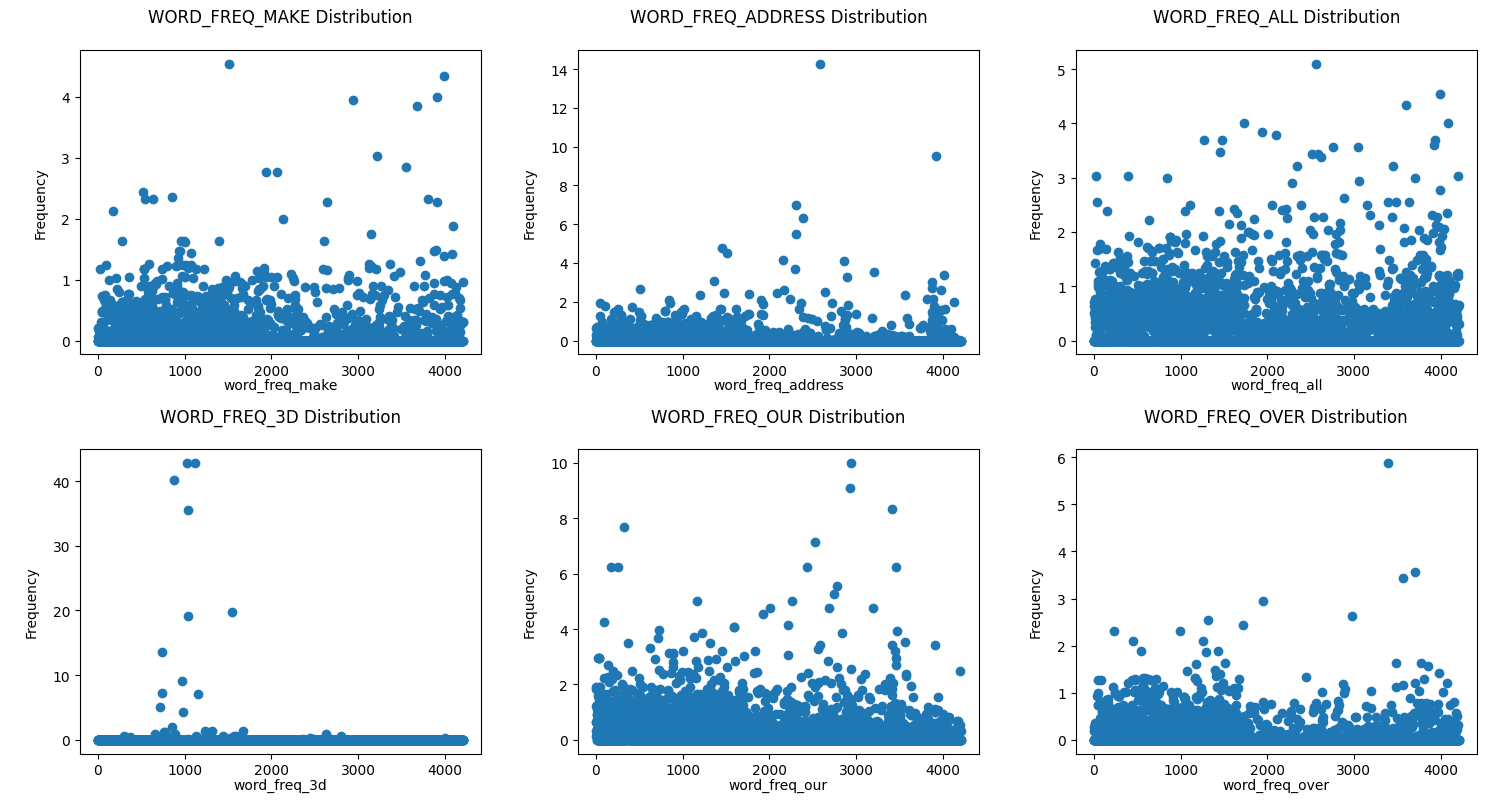
\includegraphics[width=0.65\textwidth]{spam_scatter.png}
\caption{Scatter plot}
\end{figure}

\section*{Hyperparameter Tuning Results}
\begin{table}[h!]
\centering
\renewcommand{\arraystretch}{1.3}
\begin{tabular}{|l|c|c|c|}
\hline
Model & Search Method & Best Parameters & Best CV Accuracy \\ \hline
Logistic Regression & Grid & C=1, Penalty=L1, Solver=liblinear & 0.9243 \\
SVM & Grid & C=10, Gamma=scale, Kernel=RBF & 0.9255 \\ \hline
\end{tabular}
\end{table}

%==================================================
\section*{Logistic Regression Performance}
\begin{table}[H]
\centering
\renewcommand{\arraystretch}{1.3}
\begin{tabular}{|l|c|}
\hline
Metric & Value \\ \hline
Accuracy & 0.9347 \\
Precision & 0.9297 \\
Recall & 0.9048 \\
F1 Score & 0.9170 \\
Training Time (s) & 0.0079 \\ \hline
\end{tabular}
\end{table}

%==================================================
\section*{SVM Kernel-wise Performance}
\begin{table}[h!]
\centering
\renewcommand{\arraystretch}{1.3}
\begin{tabular}{|l|c|c|c|}
\hline
Kernel & Accuracy & F1 Score & Training Time (s) \\ \hline
Linear & 0.935867 & 0.918919 & 0.215317 \\
Polynomial & 0.766033 & 0.598778 & 0.208393 \\
RBF & 0.932304 & 0.913505 & 0.111367 \\
Sigmoid & 0.896675 & 0.867580 & 0.125879 \\ \hline
\end{tabular}
\end{table}

%==================================================
\section*{K-Fold Cross-Validation Results (K = 5)}
\begin{table}[h!]
\centering
\renewcommand{\arraystretch}{1.3}
\begin{tabular}{|c|c|c|}
\hline
Fold & Logistic Regression & SVM \\ \hline
Fold 1 & 0.916914 & 0.913947 \\
Fold 2 & 0.925816 & 0.921365 \\
Fold 3 & 0.924332 & 0.921365 \\
Fold 4 & 0.921248 & 0.927192 \\
Fold 5 & 0.933135 & 0.943536 \\ \hline
Average & 0.924289 & 0.925481 \\ \hline
\end{tabular}
\end{table}

%==================================================
\section*{Comparative Analysis}

\begin{table}[H]
\centering
\renewcommand{\arraystretch}{1.3}
\begin{tabular}{|l|c|c|}
\hline
Criterion & Logistic Regression & SVM \\ \hline
Accuracy & 92.43\% & 92.55\% \\ \hline
Model Complexity & Low & High \\ \hline
Training Time & Low & High \\ \hline
Interpretability & High & Low \\ \hline
\end{tabular}
\end{table}
\section*{Performance Analysis and Discussion}

\subsection*{1. Overall Model Comparison}
In this experiment, the \textbf{Support Vector Machine (SVM)} using a Linear kernel emerged as the top performer.
\begin{itemize}
    \item \textbf{SVM (Linear Kernel):} Achieved the highest test accuracy of 0.9359 and a peak F1 score of 0.9189.
    \item \textbf{Logistic Regression:} Followed closely with an accuracy of 0.9347 and an F1 score of 0.9170.
    \item \textbf{Insight:} Both margin-based optimization and probabilistic modeling are highly effective for the Spambase dataset.
\end{itemize}

\subsection*{2. The Role of Regularization}
Regularization was pivotal in refining the Logistic Regression model.
\begin{itemize}
    \item \textbf{Optimal Setup:} The grid search identified $L1$ (Lasso) regularization with an inverse strength of $C=1$ using the \texttt{liblinear} solver.
    \item \textbf{Feature Selection:} $L1$ regularization enabled implicit feature selection by zeroing out less informative attributes.
    \item \textbf{Reliability:} A high Precision of 0.9297 indicates the model is excellent at minimizing "false positives," which is critical for preventing legitimate emails from being flagged as spam.
\end{itemize}

\subsection*{3. Impact of SVM Kernel Selection}
The choice of kernel profoundly influenced the SVM's ability to map the data.
\begin{itemize}
    \item \textbf{Linear Kernel:} Demonstrated superior performance, suggesting the features are largely linearly separable in their standardized space.
    \item \textbf{RBF Kernel:} While selected as "most stable" during tuning (CV Accuracy of 0.9255 with $C=10$), it was slightly edged out by the Linear kernel in final testing.
    \item \textbf{Polynomial Kernel:} Significantly underperformed with an accuracy of 0.7660, indicating ineffective feature mapping for this specific dataset.
\end{itemize}



\subsection*{4. Efficiency and Generalization}
An assessment of the bias-variance trade-off reveals distinct computational profiles:
\begin{itemize}
    \item \textbf{Speed:} Logistic Regression offered the lowest complexity and fastest training time (0.0079 seconds).
    \item \textbf{Complexity:} The Linear SVM was significantly more expensive, requiring 0.2153 seconds to train.
    \item \textbf{Generalization:} The consistency between Average CV scores (LR: 0.9243; SVM: 0.9255) and final test results confirms that both models generalize well to unseen data.
\end{itemize}



%==================================================
\section*{Learning Outcomes}
\begin{itemize}
    \item Understood classifiers built upon margin-based and probabilistic criterion.
    \item Applied hyperparameter tuning to improve model performance.
    \item Evaluated various models according to performance metrics.
    \item Interpreted experimental results to a throrough conclusion.
\end{itemize}

%==================================================
\section*{References}
\begin{itemize}
    \item \href{https://scikit-learn.org/stable/modules/linear_model.html#logistic-regression}{Scikit-learn: Logistic Regression}
    \item \href{https://scikit-learn.org/stable/modules/svm.html}{Scikit-learn: Support Vector Machines}
    \item \href{https://scikit-learn.org/stable/modules/grid_search.html}{Scikit-learn: Hyperparameter Optimization}
    \item \href{https://www.kaggle.com/datasets/somesh24/spambase}{Spambase Dataset – Kaggle}
    \item \href{https://archive.ics.uci.edu/ml/datasets/spambase}{UCI ML Repository – Spambase}
\end{itemize}

\end{document}
